\chapter*{Development}
\addcontentsline{toc}{chapter}{Development}
\stepcounter{chapter}

\section{Setup:}
\paragraph{Python Versions}
On my laptop (the main device for coding) I am making use of Python 3.10.5. This is because, mediapipe is not currently supported by the
later versions that are available(at this time 3/1/25 it is supported up to 3.11.0). While the version that is installed by default on
the pi is 3.13.5, I will be reducing this down to the same 3.10.5 to ensure all libraries work. To ensure there are no conflict, I will
be using a virtual environment to run my python scripts in the correct version.

\paragraph{PI OS Setup}
I am using Debian with desktop for my Pi OS version as this is the most UpToDate (and recommended for my device). I am using the desktop
version as this will allow me to more easily change code rather than using a straight Command Line interface, however, it would be
possible, and I could ssh into the Pi to execute code from there.

Initially, I did try the command-line approach, however, issues in the connection timing out and for the sake of convenience, I thought
it was best to make use of a desktop OS version.

\paragraph{Face Detection}
I am using the libraries OpenCV (Open-Source Computer Vision) and Mediapipe to detect the face and extract data. OpenCV allows me to open
the camera, read a frame and detect the existence of faces. After this, I am making use of a Mediapipe library to extract facial details. 
Using some of the bult in features these libraries provide, I then overall a triangular mesh which I can use to extract key points on the
face, such as:
\begin{itemize}
    \item Eye openness
    \item Mouth position
    \item Nose and chin locations to determine orientation / head tilt
\end{itemize}
Together, I can take video and images, and then extract the information required for me to determine
drowsiness.


\section{Data Validation}
This section is designed to break down the spread of events in a data set and ensure that there is a difference in the data, so it is
viable for training some form of AI.

\paragraph{SUST Dataset}
This refers to the ivas-University-of-Science-and-Technology-Driver-Drowsiness-Dataset \cite{SUST}
This shows an example of 5 videos for each classification (chosen at random). This is using a 2fps
sample rate.

\begin{figure}[h]
    \centering
    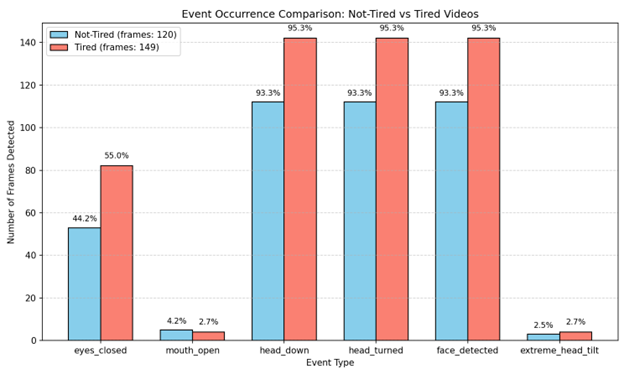
\includegraphics[width=0.9\textwidth]{Images/SUST_bar.png}
    \caption{Distribution of events in the SUST\cite{SUST} dataset}
\end{figure}

As you can see, there is a distinct difference between the 2 datasets, and so this is viable for development of an AI model. However,
surprisingly (could be just from the chosen videos) that there seems to be reduced mouth movement when tired. This was not an expected
result!

Something else that caught my eye was the number of \texttt{extreme\_head\_tilt} events. By exploring different threshold values, I was
able to determine that while tired, you tilt your head more (physically)than when awake.

However, following on from this, I formed a lightweight model where I passed in a selection of 5/6 videos of each classification and
attempted to see if these events alone were enough to form a valid model. This was a failure. This is because despite there being frames
which con-tain these tiredness events, most of the video was populated with frames which showed no at-tributes of tiredness (despite
tiredness events, a majority of the ‘normal’ frames were classi-fied as tiredness). This resulted in a poor model which had very low
confidence in its classifica-tion (52\%). Therefore, this is not a
viable strategy.

\paragraph{Bina Nusantara University}
This dataset (as discussed earlier) is a collection of images, which are labeled with “eyes closed”, “eyes open”, “yawning” and “not
yawning”.
\begin{figure}[h]
    \centering
    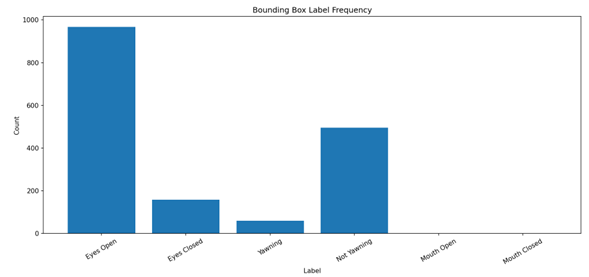
\includegraphics[width=0.9\textwidth]{Images/BINA_bar.png}
    \caption{Distribution of calssifications within the BINA\cite{BINA} dataset}
\end{figure}
These labels are purely from the pre-made labels file that comes with the data; however, I wanted to be sure that there was a range of
instances for both the tired and not tired counterparts. This suggests that there is enough variation in the dataset to potentially form
an AI model.

\section{Simple AI Models}
\subsection{Libraries}
\paragraph{TensorFlow}
Easy to use and customize. One thing I have done to help improve the computability of the project was do most of the training and coding
on my laptop, then importing the project from my Git Repository onto my pi, allowing me to train models and test more easily, rather than
trying to do it directly on the pi. Using TensorFlow, I am easily able to save models as ‘.h5’ file and then run them later.
\paragraph{TensorFlow Lite}
For ease of use and in the hope of improving running time, I will be converting my standard ‘.h5’ models into ‘.tflite’ models. This is
because general tf models are designed for training as well as inference, while tflite models are aimed more at just passing data throug
them. In the case of a Pi, this more specified computation will help to improve the return rate of the model/service, allowing me to run
it more in a given time.
This is done by compressing the models, reducing the required RAM and using a C++ runtime as opposed to the normal (more cumbersome)
python.

\subsection{Simple AI Model}
Based on my initial findings of what constitutes tiredness, I thought it best to extract the features that determine tiredness and input
their ratio values into a simple CNN model.

The model that I have used so far is comprised of 5 inputs [left eye aspect ratio, right eye aspect ratio, mouth aspect ratio, pitch, yaw]
extracted from the frame. This is then assed into a convolutional model consisting of 2 hidden layers of size 32 and 16 respectively.
This uses the ‘Adam’ (Adaptive Moment Estimation) optimiser method which adjusts weights combing the benefits of momentum and RMSProp.
On each layer the model makes use of ReLU (Rectified Linear Unit) as an activation function, allowing positive values to pass through
and negative ones to change to 0.

From this simple model, I was able to produce deduce tiredness at an accuracy of 74.5\%, based on frames extracted from the Bina
Nusantara University dataset. I believe this is because the classification of eyes open compared to eyes closed, where some examples
of training data (as well as test data) were miss labelled from the source (so it is worth wile to change these like I did to ensure
the data is classified correctly for training). This improved accuracy slightly to just over 76\%.

Following this, I thought it was a good idea to test its compatibility on the Pi and use myself as a test subject. Initially, I thought
this was working brilliantly, as closing my eyes or imitating a yawn would result in the classification of Tired (with a similar amount
of accuracy to on the testing data). However, as my testing became more extensive -- testing with varied facial expressions and
testing the effect of pitch and roll on classifications -- I noticed a discrepancy in model prediciton. As I tilted my head to the left
(moving my ear towards my shoulder), no matter the facial exression, the model predicted \textbf{tiredness}. This is something that was
completely overlooked in the testing data and implies there is a subtle trend in the data that your head tilted left is a sign of being
tired. This is a spurious correlation and could be down to camera position.

My initial thought was to retrain the model as it may be that that classifier (through that run of training) has gotten to a local
maximum (locally high bias) and been unable to recover. However, despite other iterations, I was unable to produce a more accurate model,
fluctuating between 68\% - 76\% accuracy on training data, with no more luck on testing on myself and a webcam.

From here, I thought it best to experiment with a different model to see what the upper bound in obtainable accuracy was.

\subsection{Inception Model}
This will be used to determine an upper-bound on the potential accuracy a model can give. With its primary purpose, to identify images, this is ideal.
As stated in the research section of this document, I will be proceeding with the Xception Model to classify images. The initial model I used was
pre-trained on the ImageNet dataset. This will allow for the easy identification of features (e.g. lines and shapes) without needing for the model to
learn them from scratch, which should help to improve learning rate and require less data inputs to create a fine-tuned model.
From here, I trained it on the Bina University \cite{BINA} dataset as it was composed of just images and contained a label file which would make
classification easier.

\paragraph{Issues:}
Following the training of the model, the outputs as to classifications were in the same order as they were in the labels file. As an
oversite on my part, I did not translate these labels (in the file) to English as (from the overview of the project) I could do it later.
However, during my testing, I found some of the predicted labels were not lining up with my perception of the images. For example, I
though an image was someone with their eyes closed, but the labels said otherwise. I went through I found that the dataset only had 3
classifiers in the labels, not the 4 that I had been told. From what I could understand, yawning and not yawning were translated properly,
however the eyes open/closed labels were substituted inn for a neutral face label, which has the same translation as eyes open (when
converted to English).

\paragraph{Solution:}
To fix this issue, I wrote a short section of code (based on my initial feature detection process from the data validation section) to
turn these classifications into valid labels (only for eye openness). Following this, I then went through each image, which had changed,
and verified the labeling.
Following this, I then re-trained the model on these new labels. Then I tested it on the validation dataset, resulting in 131/137
(95.6\% accuracy)  images being correctly classified. With those which were wrongly classified, I went through and had a look at where
the model was wrong. In 4 out of the 6 total images which expressed false-positives for eyes closed, I could understand why the model had
perceived the people as having their eyes closed. In the other 2 examples, one person was wearing sunglasses (which unsurprisingly)
caused an issue, with only 1 being truly wrong, classifying as eyes closed, when they were open, as well as yawning when their mouth was
only slightly open.

\noindent\rule{\textwidth}{0.4pt}

Based on these findings, I then wanted to check how the model worked on me as a use-case. To my disappointment, it was not as successful
as the validation would suggest with only around a 70\% success rate based on my attempts to fake tiredness. While I understand that my
acting abilities are not perfect, I was very surprised to find that I was not able to get a result in a similar ballpark, given that fact
my expressions were likely over-exaggerated. Additionally, when looking back through my code, in my attempt to push a working model out
before the exam season began, I have noticed that I had not altered or included the variations to input data, like I had in the Simple
Convolutional AI models.
As expected, after adding in the variations to:
\begin{itemize}
	\item Brightness
	\item Contrast
	\item Saturation
	\item Flipping the image
\end{itemize}
,the accuracy of the model has decreased (relative to the testing set), with the hope that it is more versatile for a wider variety of
end implementations. With a 75.91\% accuracy (104/137) on the Bina University dataset resulting in correct predictions, this was more of
a detriment than I predicted.

\subsection{Dataset Resolution}
While the previous model was reasonably accurate on determining if the user had their eyes open/closed or if you were yawning or not,
it would require an additional threshold to determine tiredness from this. In my earlier model versions, I determined the classifications
of eyes closed or yawning as a positive case of tiredness. However, with the Xception model taking in image inputs, I wanted to experiment
with opinionated learning. This would allow me to define the dataset based on my opinion of someone looking tired and considering a larger
array of features such as:
\begin{itemize}
	\item Eyes open (but not fully), implying they are drained
	\item Bags under the eyes
	\item Mouth positions for talking vs yawning
\end{itemize}
,with this in mind, I decided to go through manually re-classifying the data and re-train several models on this.
One of the things to consider when doing this is opinion. Since I am classifying the data, my opinion may be different to someone else,
which can lead to inconsistencies based on person classifying because of a larger array of external factors.
With this being an opinion and not necessarily a definitive solution yes or no, there was a slight reduction in accuracy to 73.72\%
(only a 2.19\% loss compared to the previous model which used definitive classifications); far better than I could have hoped, for with
an 85.33\% accuracy in detecting ‘alertness’.

\paragraph{Personal Testing:}
Following my previous tests on myself, I found that I would try and remove personal bias to a favorable model by formulating a
quantitative dataset that I can test against. While only consisting of 100 images and a fixed environment, I wanted to test model
robustness thorugh varying facial expressions.
Despite using a webcam and in my room with no natural light and unlikely camera placement (vastly different from the actual use case),
I was still able to obtain a 63.27\% accuracy in detecting ‘tiredness’. From the results, however, all errors were False Positives for
alertness (mistaking the user for being alert compared to tired). This could be down to a variety of factors:
\begin{itemize}
    \item \textbf{Camera Placement:} With the camera being mounted ontop of my monitor (standard webcamera location), it was directly
    in the line--of--sight. This minute change could result in my eyes being more correctly orientated for an Alert classification.
    \item \textbf{Lighting:} To reduce discrepancy caused by glare, I aimed to produce a high contrast image by removing background
    light and to reduce the effect of external factors. However, this lack of ambient light and harsh gradients could have formed an environment
    that lies outside of the training distribution.
\end{itemize}

Following on from this, it would be more ideal to generate testing data in the correct working environment to get a more accurate representation
of the models predictive capabilities. Additionally, the effect of background lighting and camera placement might also be affecting the model
and so a more extensive and varied dataset might be more representative of overall performance.